\documentclass[]{book}
\usepackage{lmodern}
\usepackage{amssymb,amsmath}
\usepackage{ifxetex,ifluatex}
\usepackage{fixltx2e} % provides \textsubscript
\ifnum 0\ifxetex 1\fi\ifluatex 1\fi=0 % if pdftex
  \usepackage[T1]{fontenc}
  \usepackage[utf8]{inputenc}
\else % if luatex or xelatex
  \ifxetex
    \usepackage{mathspec}
  \else
    \usepackage{fontspec}
  \fi
  \defaultfontfeatures{Ligatures=TeX,Scale=MatchLowercase}
\fi
% use upquote if available, for straight quotes in verbatim environments
\IfFileExists{upquote.sty}{\usepackage{upquote}}{}
% use microtype if available
\IfFileExists{microtype.sty}{%
\usepackage{microtype}
\UseMicrotypeSet[protrusion]{basicmath} % disable protrusion for tt fonts
}{}
\usepackage[margin=1in]{geometry}
\usepackage{hyperref}
\hypersetup{unicode=true,
            pdftitle={Data Analytics in RStudio},
            pdfauthor={Gaurav Satav},
            pdfborder={0 0 0},
            breaklinks=true}
\urlstyle{same}  % don't use monospace font for urls
\usepackage{natbib}
\bibliographystyle{apalike}
\usepackage{color}
\usepackage{fancyvrb}
\newcommand{\VerbBar}{|}
\newcommand{\VERB}{\Verb[commandchars=\\\{\}]}
\DefineVerbatimEnvironment{Highlighting}{Verbatim}{commandchars=\\\{\}}
% Add ',fontsize=\small' for more characters per line
\usepackage{framed}
\definecolor{shadecolor}{RGB}{248,248,248}
\newenvironment{Shaded}{\begin{snugshade}}{\end{snugshade}}
\newcommand{\KeywordTok}[1]{\textcolor[rgb]{0.13,0.29,0.53}{\textbf{#1}}}
\newcommand{\DataTypeTok}[1]{\textcolor[rgb]{0.13,0.29,0.53}{#1}}
\newcommand{\DecValTok}[1]{\textcolor[rgb]{0.00,0.00,0.81}{#1}}
\newcommand{\BaseNTok}[1]{\textcolor[rgb]{0.00,0.00,0.81}{#1}}
\newcommand{\FloatTok}[1]{\textcolor[rgb]{0.00,0.00,0.81}{#1}}
\newcommand{\ConstantTok}[1]{\textcolor[rgb]{0.00,0.00,0.00}{#1}}
\newcommand{\CharTok}[1]{\textcolor[rgb]{0.31,0.60,0.02}{#1}}
\newcommand{\SpecialCharTok}[1]{\textcolor[rgb]{0.00,0.00,0.00}{#1}}
\newcommand{\StringTok}[1]{\textcolor[rgb]{0.31,0.60,0.02}{#1}}
\newcommand{\VerbatimStringTok}[1]{\textcolor[rgb]{0.31,0.60,0.02}{#1}}
\newcommand{\SpecialStringTok}[1]{\textcolor[rgb]{0.31,0.60,0.02}{#1}}
\newcommand{\ImportTok}[1]{#1}
\newcommand{\CommentTok}[1]{\textcolor[rgb]{0.56,0.35,0.01}{\textit{#1}}}
\newcommand{\DocumentationTok}[1]{\textcolor[rgb]{0.56,0.35,0.01}{\textbf{\textit{#1}}}}
\newcommand{\AnnotationTok}[1]{\textcolor[rgb]{0.56,0.35,0.01}{\textbf{\textit{#1}}}}
\newcommand{\CommentVarTok}[1]{\textcolor[rgb]{0.56,0.35,0.01}{\textbf{\textit{#1}}}}
\newcommand{\OtherTok}[1]{\textcolor[rgb]{0.56,0.35,0.01}{#1}}
\newcommand{\FunctionTok}[1]{\textcolor[rgb]{0.00,0.00,0.00}{#1}}
\newcommand{\VariableTok}[1]{\textcolor[rgb]{0.00,0.00,0.00}{#1}}
\newcommand{\ControlFlowTok}[1]{\textcolor[rgb]{0.13,0.29,0.53}{\textbf{#1}}}
\newcommand{\OperatorTok}[1]{\textcolor[rgb]{0.81,0.36,0.00}{\textbf{#1}}}
\newcommand{\BuiltInTok}[1]{#1}
\newcommand{\ExtensionTok}[1]{#1}
\newcommand{\PreprocessorTok}[1]{\textcolor[rgb]{0.56,0.35,0.01}{\textit{#1}}}
\newcommand{\AttributeTok}[1]{\textcolor[rgb]{0.77,0.63,0.00}{#1}}
\newcommand{\RegionMarkerTok}[1]{#1}
\newcommand{\InformationTok}[1]{\textcolor[rgb]{0.56,0.35,0.01}{\textbf{\textit{#1}}}}
\newcommand{\WarningTok}[1]{\textcolor[rgb]{0.56,0.35,0.01}{\textbf{\textit{#1}}}}
\newcommand{\AlertTok}[1]{\textcolor[rgb]{0.94,0.16,0.16}{#1}}
\newcommand{\ErrorTok}[1]{\textcolor[rgb]{0.64,0.00,0.00}{\textbf{#1}}}
\newcommand{\NormalTok}[1]{#1}
\usepackage{longtable,booktabs}
\usepackage{graphicx,grffile}
\makeatletter
\def\maxwidth{\ifdim\Gin@nat@width>\linewidth\linewidth\else\Gin@nat@width\fi}
\def\maxheight{\ifdim\Gin@nat@height>\textheight\textheight\else\Gin@nat@height\fi}
\makeatother
% Scale images if necessary, so that they will not overflow the page
% margins by default, and it is still possible to overwrite the defaults
% using explicit options in \includegraphics[width, height, ...]{}
\setkeys{Gin}{width=\maxwidth,height=\maxheight,keepaspectratio}
\IfFileExists{parskip.sty}{%
\usepackage{parskip}
}{% else
\setlength{\parindent}{0pt}
\setlength{\parskip}{6pt plus 2pt minus 1pt}
}
\setlength{\emergencystretch}{3em}  % prevent overfull lines
\providecommand{\tightlist}{%
  \setlength{\itemsep}{0pt}\setlength{\parskip}{0pt}}
\setcounter{secnumdepth}{5}
% Redefines (sub)paragraphs to behave more like sections
\ifx\paragraph\undefined\else
\let\oldparagraph\paragraph
\renewcommand{\paragraph}[1]{\oldparagraph{#1}\mbox{}}
\fi
\ifx\subparagraph\undefined\else
\let\oldsubparagraph\subparagraph
\renewcommand{\subparagraph}[1]{\oldsubparagraph{#1}\mbox{}}
\fi

%%% Use protect on footnotes to avoid problems with footnotes in titles
\let\rmarkdownfootnote\footnote%
\def\footnote{\protect\rmarkdownfootnote}

%%% Change title format to be more compact
\usepackage{titling}

% Create subtitle command for use in maketitle
\newcommand{\subtitle}[1]{
  \posttitle{
    \begin{center}\large#1\end{center}
    }
}

\setlength{\droptitle}{-2em}
  \title{Data Analytics in RStudio}
  \pretitle{\vspace{\droptitle}\centering\huge}
  \posttitle{\par}
  \author{Gaurav Satav}
  \preauthor{\centering\large\emph}
  \postauthor{\par}
  \predate{\centering\large\emph}
  \postdate{\par}
  \date{2018-02-22}

\usepackage{booktabs}

\usepackage{amsthm}
\newtheorem{theorem}{Theorem}[chapter]
\newtheorem{lemma}{Lemma}[chapter]
\theoremstyle{definition}
\newtheorem{definition}{Definition}[chapter]
\newtheorem{corollary}{Corollary}[chapter]
\newtheorem{proposition}{Proposition}[chapter]
\theoremstyle{definition}
\newtheorem{example}{Example}[chapter]
\theoremstyle{definition}
\newtheorem{exercise}{Exercise}[chapter]
\theoremstyle{remark}
\newtheorem*{remark}{Remark}
\newtheorem*{solution}{Solution}
\begin{document}
\maketitle

{
\setcounter{tocdepth}{1}
\tableofcontents
}
\chapter*{Preface}\label{preface}
\addcontentsline{toc}{chapter}{Preface}

This document is an attempt to provide the reader with a walkthrough
into how a typical analysis is carried out using R Studios.

\chapter{Introduction}\label{introduction}

Its hard to ignore the strides currently made in the direction

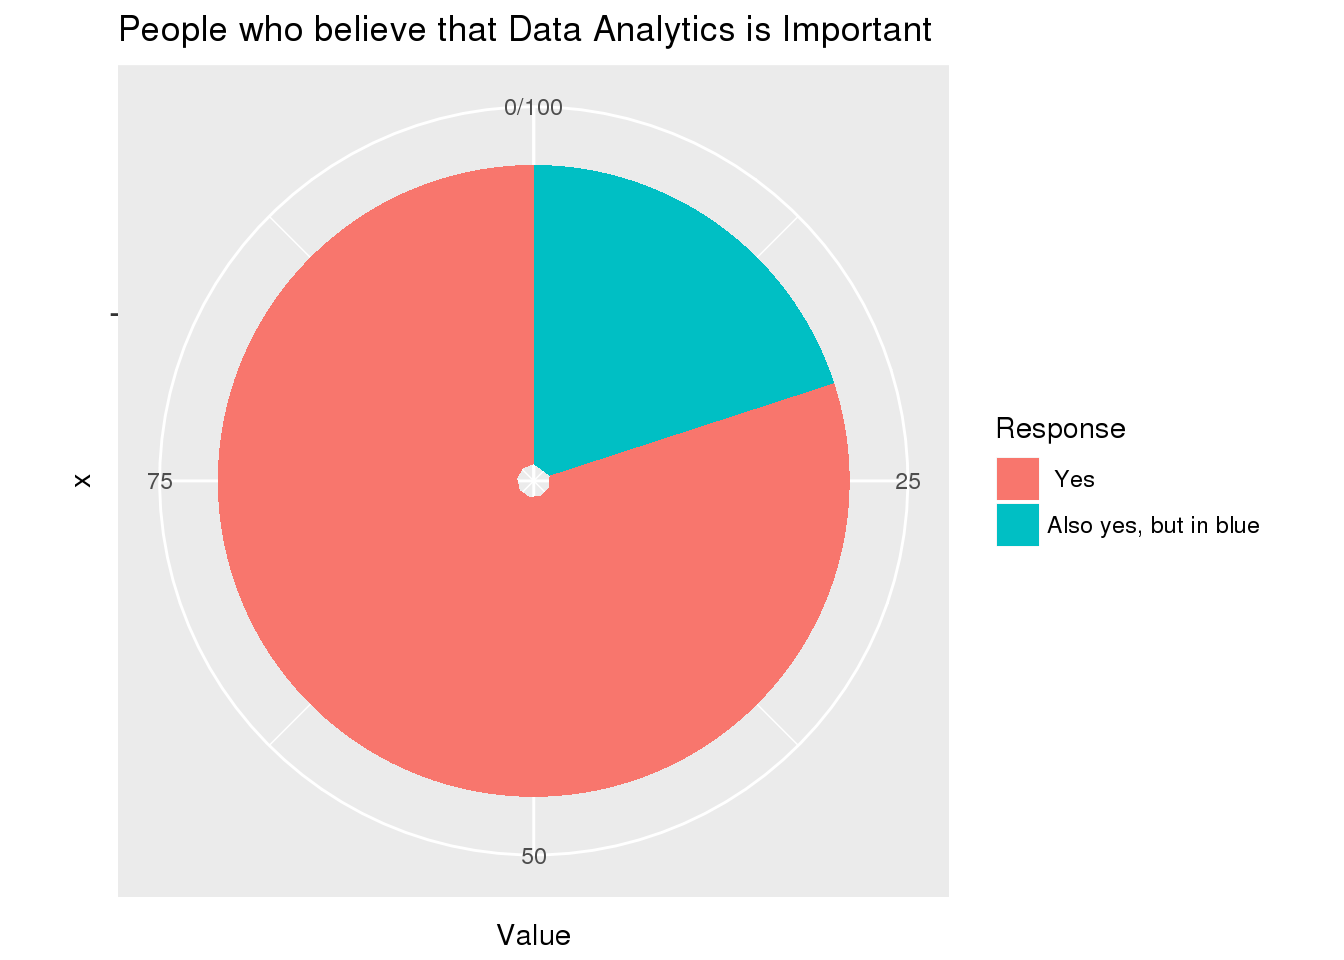
\includegraphics{01-Introduction_files/figure-latex/yesno-1.pdf}

\section{The R Language}\label{the-r-language}

R is a free software environment for statistical computing and graphics.
It compiles and runs on a wide variety of UNIX platforms, Windows and
MacOS.

\textbf{The R environment}

R is an integrated suite of software facilities for data manipulation,
calculation and graphical display. Among other things it has

\begin{itemize}
\tightlist
\item
  an effective data handling and storage facility,
\item
  a suite of operators for calculations on arrays, in particular
  matrices,
\item
  a large, coherent, integrated collection of intermediate tools for
  data analysis,
\item
  graphical facilities for data analysis and display either directly at
  the computer or on hardcopy, and
\item
  a well developed, simple and effective programming language (called
  `S') which includes conditionals, loops, user defined recursive
  functions and input and output facilities. (Indeed most of the system
  supplied functions are themselves written in the S language.)
\end{itemize}

The term ``environment'' is intended to characterize it as a fully
planned and coherent system, rather than an incremental accretion of
very specific and inflexible tools, as is frequently the case with other
data analysis software.

R is very much a vehicle for newly developing methods of interactive
data analysis. It has developed rapidly, and has been extended by a
large collection of packages. However, most programs written in R are
essentially ephemeral, written for a single piece of data analysis.

You can get yourself aquainted with the basics of R by visiting this
\href{https://cran.r-project.org/doc/manuals/r-release/R-intro.html}{link}

You can download R by clicking the
\href{https://cran.r-project.org/}{link here}.

\section{R Studios}\label{r-studios}

RStudio is an integrated development environment (IDE) for R. It
includes a console, syntax-highlighting editor that supports direct code
execution, as well as tools for plotting, history, debugging and
workspace management.

RStudio is available in open source and commercial editions and runs on
the desktop (Windows, Mac, and Linux) or in a browser connected to
RStudio Server or RStudio Server Pro (Debian/Ubuntu, RedHat/CentOS, and
SUSE Linux).

\begin{figure}
\centering
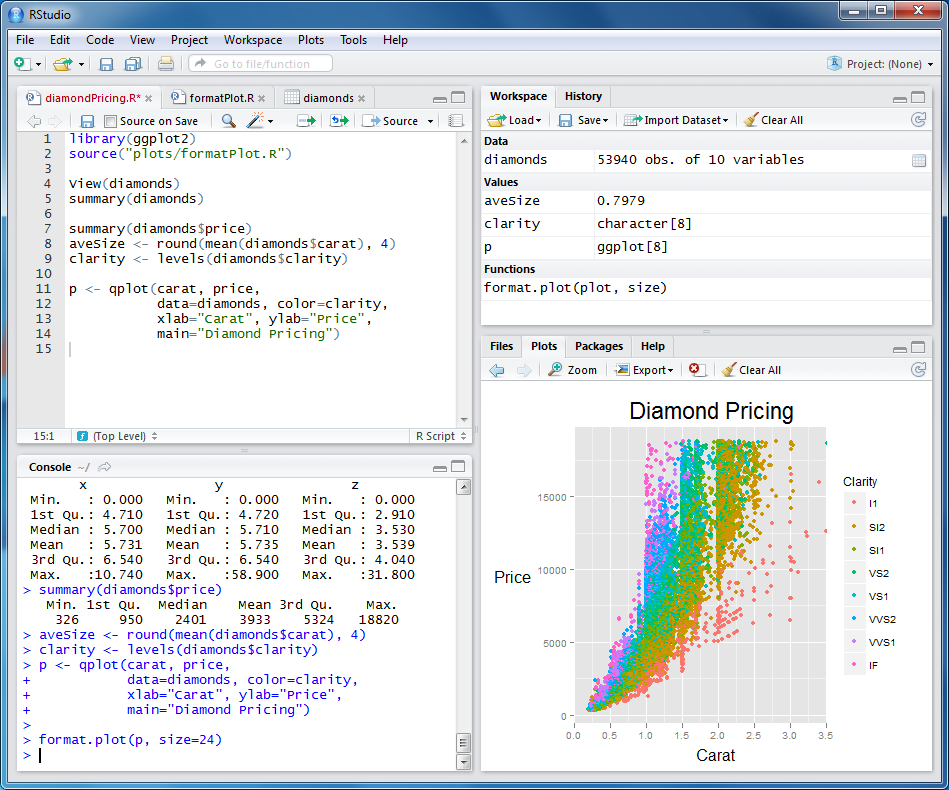
\includegraphics{./images/RStudio-Screenshot.png}
\caption{}
\end{figure}

\textbf{Downloading R Studios}

\begin{itemize}
\tightlist
\item
  Before downloading R Studios make sure you have R installed on your
  system. If not the refer the previous page for the link
\end{itemize}

Basically there are two version of RStudio (
\href{https://support.rstudio.com/hc/en-us/articles/217799198-What-is-the-difference-between-RStudio-Desktop-and-RStudio-Server-}{whats
the difference?} )

\begin{itemize}
\item
  Desktop Version
\item
  Server Version
\end{itemize}

We recommend installation of the server version or R Studio and once its
installed we can access it using our browser at port 8787

Click here to
\href{https://www.rstudio.com/products/rstudio/download-server/}{install
R Studio} for linux.

\chapter{Setting up a Project}\label{setting-up-a-project}

Before we start with our analysis, we'll start off by setting up a
project. Setting up a project helps us in the following ways

\begin{itemize}
\tightlist
\item
  Keeping track of all the files and variables which are created in
  between our executions.
\item
  It also helps us to reproduce our work and keep a track of all the
  libraries upon which our code relies upon (see
  \href{https://github.com/rstudio/packrat}{\texttt{packrat}}).
\item
  It allows us to enable version control.
\end{itemize}

\section{Github Integration}\label{github-integration}

Version control helps software teams manage changes to source code over
time. Version control software keeps track of every modification to the
code in a special kind of database. If a mistake is made, developers can
turn back the clock and compare earlier versions of the code to help fix
the mistake while minimizing disruption to all team members. Version
control systems have been around for a long time but continue to
increase in popularity with data science workflows.

The RStudio IDE has integrated support for version control which would
help us keep track of our changes and push them onto Github.

\textbf{Additional Resource} -
\href{https://support.rstudio.com/hc/en-us/articles/200532077-Version-Control-with-Git-and-SVN}{Using
Version Control with RStudio}

\chapter{Preparing the Canvas}\label{preparing-the-canvas}

Consider the following scenario, you are asked to perform analysis on
some data, we would all agree that it would be a tedious task to
complete our analysis using the command line interface. The RStudio IDE
(or any IDE for that matter) provides us with the freedom to reproduce
the execution of our code sequentially to be executed on someone else
along with host of other important advantage.

Now as it happens at the end of most analysis we are required to produce
a report to be shared. This report in general takes one of the following
forms.

\begin{itemize}
\tightlist
\item
  A Spreadsheet.
\item
  A text document.
\item
  A powerpoint presentation.
\end{itemize}

thinking on similar lines as we did while comparing the \emph{CMD line}
to a \emph{text editor} we see that it would really be a tedious job to
produce reports especially if the reports are going to be repetative and
similar in nature.Before we start writing a single line of code, I
encourage you to ask yourself, \emph{what is my output file format going
to be ?}.

\textbf{Beginning at the end.}

R Studio provides us with the following (along with many other) output
formats in which we can share our analysis.

\begin{itemize}
\tightlist
\item
  R Markdown
\item
  Dashboards
\item
  Web Pages (Blogs and Books)
\item
  Web Applications
\end{itemize}

We'll skim on the surface of each of these output formats in the
following chapters.

\section{R Markdown}\label{r-markdown}

This is an R Markdown document. Markdown is a simple formatting syntax
for authoring HTML, PDF, and MS Word documents. For more details on
using R Markdown see \url{http://rmarkdown.rstudio.com}.

When you click the \textbf{Knit} button a document will be generated
that includes both content as well as the output of any embedded R code
chunks within the document. You can embed an R code chunk like this:

\begin{Shaded}
\begin{Highlighting}[]
\KeywordTok{summary}\NormalTok{(cars)}
\end{Highlighting}
\end{Shaded}

\begin{verbatim}
##      speed           dist       
##  Min.   : 4.0   Min.   :  2.00  
##  1st Qu.:12.0   1st Qu.: 26.00  
##  Median :15.0   Median : 36.00  
##  Mean   :15.4   Mean   : 42.98  
##  3rd Qu.:19.0   3rd Qu.: 56.00  
##  Max.   :25.0   Max.   :120.00
\end{verbatim}

\subsubsection{Including Plots}\label{including-plots}

You can also embed plots, for example:

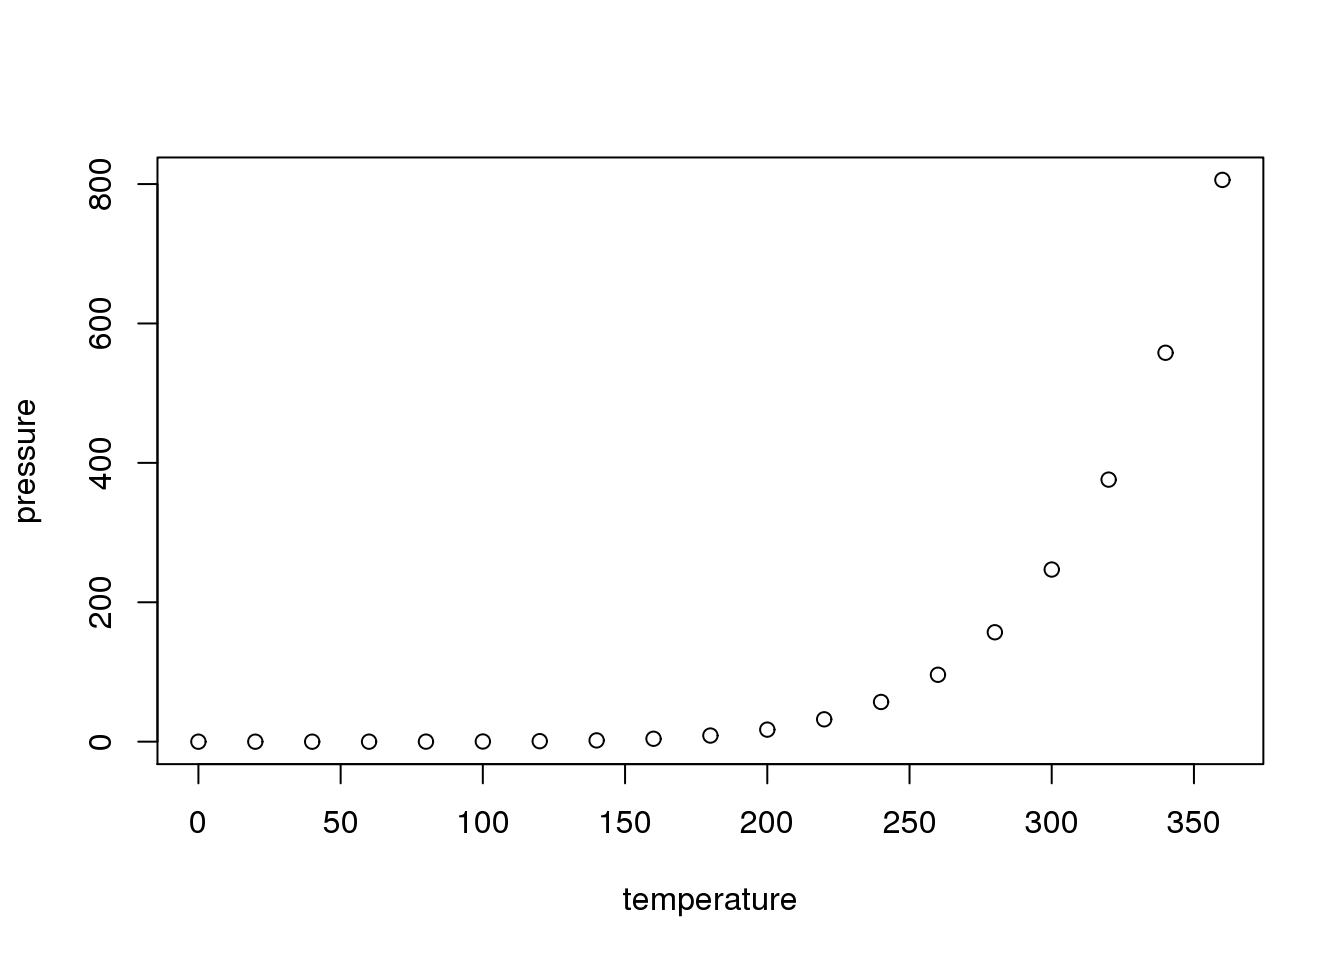
\includegraphics{07-RMarkdown_files/figure-latex/pressure-1.pdf}

Note that the \texttt{echo\ =\ FALSE} parameter was added to the code
chunk to prevent printing of the R code that generated the plot.

\section{Dashboards}\label{dashboards}

Dashboards are a great tool to represent live data or data in forms of
reports. The
\href{http://rmarkdown.rstudio.com/flexdashboard/}{\texttt{flexdashboard}}
library allows us to do just that. It enables you to easily create
flexible, attractive, interactive dashboards with R. Authoring and
customization of dashboards is done using
\href{http://rmarkdown.rstudio.com/}{R Markdown} and you can optionally
include \href{http://shiny.rstudio.com/}{Shiny}(more on it later)
components for additional interactivity.

Highlights of the flexdashboard package include:

\begin{itemize}
\item
  Support for a wide variety of components including interactive
  htmlwidgets; base, lattice, and grid graphics; tabular data; gauges;
  and value boxes.
\item
  Flexible and easy to specify row and column-based layouts. Components
  are intelligently re-sized to fill the browser and adapted for display
  on mobile devices.
\item
  Extensive support for text annotations to include assumptions,
  contextual narrative, and analysis within dashboards.
\item
  Storyboard layouts for presenting sequences of visualizations and
  related commentary.
\item
  By default dashboards are standard HTML documents that can be deployed
  on any web server or even attached to an email message. You can
  optionally add Shiny components for additional interactivity and then
  deploy on Shiny Server or shinyapps.io.
\end{itemize}

You can explore the gallery of the dashboards at
\url{https://rmarkdown.rstudio.com/flexdashboard/examples.html}

Additional learning resource is
\href{https://blog.rstudio.com/2016/05/17/flexdashboard-easy-interactive-dashboards-for-r/}{here}

\section{Blog}\label{blog}

It so often happens that we continue to learn new things and and more
often than not, forget them due to one reason or the other. Maintaining
a blog helps us to write in our own words what it is that we've learned
and also it can help you showcase your knowledge to someone when asked
upon.

\textbf{Blogdown} is an awesome tool developed by Yihui Xi which makes
our lives a whole lot easier to create, maintain and update our own
blog. Its a bit of a trouble at start, but once you get going you come
to see its effectiveness.

Once we create our blog we can then choose to host it either on Github
Pages or on Netlify.

\textbf{Additional Resources}

\begin{itemize}
\tightlist
\item
  \href{https://bookdown.org/yihui/blogdown/}{blogdown: Creating
  Websites with R Markdown}
\item
  \href{https://tclavelle.github.io/blog/blogdown_github/}{Building a
  blog with blogdown}
\end{itemize}

\section{Books}\label{books}

Similar to the \texttt{blogdown} package, \texttt{bookdown} as the name
suggest is used for writing books. The book you're currently reading was
written using the same package.

\textbf{Additional Resources} -
\href{https://bookdown.org/yihui/bookdown/}{bookdown: Authoring Books
and Technical Documents with R Markdown}

\section{Web Applications.}\label{web-applications.}

Shiny is an R package that makes it easy to build interactive web
applications (apps) straight from R.

A simple example of the application is seen
\href{https://gauravsatav.shinyapps.io/WebApp/}{here}

This application is hosted on the \url{https://www.shinyapps.io/} server
\href{https://www.shinyapps.io/admin/\#/application/239302}{.}

\textbf{Additional Resources}

\begin{itemize}
\tightlist
\item
  \href{https://shiny.rstudio.com/tutorial/}{Learn Shiny}
\end{itemize}

\chapter{Getting to work}\label{getting-to-work}

There is a problem hosted on \href{https://www.kaggle.com/}{Kaggle} (a
platform which hosts many predictive modelling and analytics
competitions) knows as the
\href{https://www.kaggle.com/c/titanic}{Titanic: Machine Learning from
Disaster}.

In this competitions, we are asked to predict whether a given set
passenger survived or died in the sinking of RMS Titanic.

We'll now start our walkthrough. All credits for the

\section{Once upon a time\ldots{}}\label{once-upon-a-time}

The sinking of the RMS Titanic is one of the most infamous shipwrecks in
history. On April 15, 1912, during her maiden voyage, the Titanic sank
after colliding with an iceberg, killing 1502 out of 2224 passengers and
crew. This sensational tragedy shocked the international community and
led to better safety regulations for ships.

One of the reasons that the shipwreck led to such loss of life was that
there were not enough lifeboats for the passengers and crew. Although
there was some element of luck involved in surviving the sinking, some
groups of people were more likely to survive than others, such as women,
children, and the upper-class.

\section{Load and check data}\label{load-and-check-data}

\begin{Shaded}
\begin{Highlighting}[]
\CommentTok{# Load packages}

\CommentTok{# Base Package}
\KeywordTok{library}\NormalTok{(}\StringTok{'base'}\NormalTok{)}

\CommentTok{# Visualization}
\KeywordTok{library}\NormalTok{(}\StringTok{'ggplot2'}\NormalTok{)}
\KeywordTok{library}\NormalTok{(}\StringTok{'ggthemes'}\NormalTok{)}
\KeywordTok{library}\NormalTok{(}\StringTok{'scales'}\NormalTok{)}

\CommentTok{# Data Manipulation}
\KeywordTok{library}\NormalTok{(}\StringTok{'dplyr'}\NormalTok{) }

\CommentTok{# Imputation}
\KeywordTok{library}\NormalTok{(}\StringTok{'mice'}\NormalTok{) }

\CommentTok{# Classification algorithm}
\KeywordTok{library}\NormalTok{(}\StringTok{'randomForest'}\NormalTok{) }
\end{Highlighting}
\end{Shaded}

Now that our packages are loaded, let's read in and take a peek at the
data.

\begin{Shaded}
\begin{Highlighting}[]
\NormalTok{train <-}\StringTok{ }\KeywordTok{read.csv}\NormalTok{(}\StringTok{'./input/train.csv'}\NormalTok{, }\DataTypeTok{stringsAsFactors =}\NormalTok{ F)}
\NormalTok{test  <-}\StringTok{ }\KeywordTok{read.csv}\NormalTok{(}\StringTok{'./input/test.csv'}\NormalTok{, }\DataTypeTok{stringsAsFactors =}\NormalTok{ F)}

\NormalTok{full  <-}\StringTok{ }\KeywordTok{bind_rows}\NormalTok{(train, test) }\CommentTok{# bind training & test data}

\CommentTok{# check data}
\KeywordTok{str}\NormalTok{(full)}
\end{Highlighting}
\end{Shaded}

\begin{verbatim}
## 'data.frame':    1309 obs. of  12 variables:
##  $ PassengerId: int  1 2 3 4 5 6 7 8 9 10 ...
##  $ Survived   : int  0 1 1 1 0 0 0 0 1 1 ...
##  $ Pclass     : int  3 1 3 1 3 3 1 3 3 2 ...
##  $ Name       : chr  "Braund, Mr. Owen Harris" "Cumings, Mrs. John Bradley (Florence Briggs Thayer)" "Heikkinen, Miss. Laina" "Futrelle, Mrs. Jacques Heath (Lily May Peel)" ...
##  $ Sex        : chr  "male" "female" "female" "female" ...
##  $ Age        : num  22 38 26 35 35 NA 54 2 27 14 ...
##  $ SibSp      : int  1 1 0 1 0 0 0 3 0 1 ...
##  $ Parch      : int  0 0 0 0 0 0 0 1 2 0 ...
##  $ Ticket     : chr  "A/5 21171" "PC 17599" "STON/O2. 3101282" "113803" ...
##  $ Fare       : num  7.25 71.28 7.92 53.1 8.05 ...
##  $ Cabin      : chr  "" "C85" "" "C123" ...
##  $ Embarked   : chr  "S" "C" "S" "S" ...
\end{verbatim}

We've got a sense of our variables, their class type, and the first few
observations of each. We know we're working with 1309 observations of 12
variables. To make things a bit more explicit since a couple of the
variable names aren't 100\% illuminating, here's what we've got to deal
with:

\section{Feature Engineering}\label{feature-engineering}

\subsection{What's in a name?}\label{whats-in-a-name}

The first variable which catches my attention is passenger name because
we can break it down into additional meaningful variables which can feed
predictions or be used in the creation of additional new variables. For
instance, passenger title is contained within the passenger name
variable and we can use surname to represent families. Let's do some
feature engineering!

\begin{Shaded}
\begin{Highlighting}[]
\CommentTok{# Grab title from passenger names}
\NormalTok{full}\OperatorTok{$}\NormalTok{Title <-}\StringTok{ }\KeywordTok{gsub}\NormalTok{(}\StringTok{'(.*, )|(}\CharTok{\textbackslash{}\textbackslash{}}\StringTok{..*)'}\NormalTok{, }\StringTok{''}\NormalTok{, full}\OperatorTok{$}\NormalTok{Name)}

\CommentTok{# Show title counts by sex}
\KeywordTok{table}\NormalTok{(full}\OperatorTok{$}\NormalTok{Sex, full}\OperatorTok{$}\NormalTok{Title)}
\end{Highlighting}
\end{Shaded}

\begin{verbatim}
##         
##          Capt Col Don Dona  Dr Jonkheer Lady Major Master Miss Mlle Mme
##   female    0   0   0    1   1        0    1     0      0  260    2   1
##   male      1   4   1    0   7        1    0     2     61    0    0   0
##         
##           Mr Mrs  Ms Rev Sir the Countess
##   female   0 197   2   0   0            1
##   male   757   0   0   8   1            0
\end{verbatim}

\begin{Shaded}
\begin{Highlighting}[]
\CommentTok{# Titles with very low cell counts to be combined to "rare" level}
\NormalTok{rare_title <-}\StringTok{ }\KeywordTok{c}\NormalTok{(}\StringTok{'Dona'}\NormalTok{, }\StringTok{'Lady'}\NormalTok{, }\StringTok{'the Countess'}\NormalTok{,}\StringTok{'Capt'}\NormalTok{, }\StringTok{'Col'}\NormalTok{, }\StringTok{'Don'}\NormalTok{, }
                \StringTok{'Dr'}\NormalTok{, }\StringTok{'Major'}\NormalTok{, }\StringTok{'Rev'}\NormalTok{, }\StringTok{'Sir'}\NormalTok{, }\StringTok{'Jonkheer'}\NormalTok{)}

\CommentTok{# Also reassign mlle, ms, and mme accordingly}
\NormalTok{full}\OperatorTok{$}\NormalTok{Title[full}\OperatorTok{$}\NormalTok{Title }\OperatorTok{==}\StringTok{ 'Mlle'}\NormalTok{]        <-}\StringTok{ 'Miss'} 
\NormalTok{full}\OperatorTok{$}\NormalTok{Title[full}\OperatorTok{$}\NormalTok{Title }\OperatorTok{==}\StringTok{ 'Ms'}\NormalTok{]          <-}\StringTok{ 'Miss'}
\NormalTok{full}\OperatorTok{$}\NormalTok{Title[full}\OperatorTok{$}\NormalTok{Title }\OperatorTok{==}\StringTok{ 'Mme'}\NormalTok{]         <-}\StringTok{ 'Mrs'} 
\NormalTok{full}\OperatorTok{$}\NormalTok{Title[full}\OperatorTok{$}\NormalTok{Title }\OperatorTok\StringTok{ }\NormalTok{rare_title]  <-}\StringTok{ 'Rare Title'}

\CommentTok{# Show title counts by sex again}
\KeywordTok{table}\NormalTok{(full}\OperatorTok{$}\NormalTok{Sex, full}\OperatorTok{$}\NormalTok{Title)}
\end{Highlighting}
\end{Shaded}

\begin{verbatim}
##         
##          Master Miss  Mr Mrs Rare Title
##   female      0  264   0 198          4
##   male       61    0 757   0         25
\end{verbatim}

\begin{Shaded}
\begin{Highlighting}[]
\CommentTok{# Finally, grab surname from passenger name}
\NormalTok{full}\OperatorTok{$}\NormalTok{Surname <-}\StringTok{ }\KeywordTok{sapply}\NormalTok{(full}\OperatorTok{$}\NormalTok{Name,  }
                      \ControlFlowTok{function}\NormalTok{(x) }\KeywordTok{strsplit}\NormalTok{(x, }\DataTypeTok{split =} \StringTok{'[,.]'}\NormalTok{)[[}\DecValTok{1}\NormalTok{]][}\DecValTok{1}\NormalTok{])}
\end{Highlighting}
\end{Shaded}

We have 875 unique surnames. I would be interested to infer ethnicity
based on surname --- another time.

\subsection{Do families sink or swim
together?}\label{do-families-sink-or-swim-together}

Now that we've taken care of splitting passenger name into some new
variables, we can take it a step further and make some new family
variables. First we're going to make a family size variable based on
number of siblings/spouse(s) (maybe someone has more than one spouse?)
and number of children/parents.

\begin{Shaded}
\begin{Highlighting}[]
\CommentTok{# Create a family size variable including the passenger themselves}
\NormalTok{full}\OperatorTok{$}\NormalTok{Fsize <-}\StringTok{ }\NormalTok{full}\OperatorTok{$}\NormalTok{SibSp }\OperatorTok{+}\StringTok{ }\NormalTok{full}\OperatorTok{$}\NormalTok{Parch }\OperatorTok{+}\StringTok{ }\DecValTok{1}

\CommentTok{# Create a family variable }
\NormalTok{full}\OperatorTok{$}\NormalTok{Family <-}\StringTok{ }\KeywordTok{paste}\NormalTok{(full}\OperatorTok{$}\NormalTok{Surname, full}\OperatorTok{$}\NormalTok{Fsize, }\DataTypeTok{sep=}\StringTok{'_'}\NormalTok{)}
\end{Highlighting}
\end{Shaded}

What does our family size variable look like? To help us understand how
it may relate to survival, let's plot it among the training data.

\begin{Shaded}
\begin{Highlighting}[]
\CommentTok{# Use ggplot2 to visualize the relationship between family size & survival}
\KeywordTok{ggplot}\NormalTok{(full[}\DecValTok{1}\OperatorTok{:}\DecValTok{891}\NormalTok{,], }\KeywordTok{aes}\NormalTok{(}\DataTypeTok{x =}\NormalTok{ Fsize, }\DataTypeTok{fill =} \KeywordTok{factor}\NormalTok{(Survived))) }\OperatorTok{+}
\StringTok{  }\KeywordTok{geom_bar}\NormalTok{(}\DataTypeTok{stat=}\StringTok{'count'}\NormalTok{, }\DataTypeTok{position=}\StringTok{'dodge'}\NormalTok{) }\OperatorTok{+}
\StringTok{  }\KeywordTok{scale_x_continuous}\NormalTok{(}\DataTypeTok{breaks=}\KeywordTok{c}\NormalTok{(}\DecValTok{1}\OperatorTok{:}\DecValTok{11}\NormalTok{)) }\OperatorTok{+}
\StringTok{  }\KeywordTok{labs}\NormalTok{(}\DataTypeTok{x =} \StringTok{'Family Size'}\NormalTok{) }\OperatorTok{+}
\StringTok{  }\KeywordTok{theme_few}\NormalTok{()}
\end{Highlighting}
\end{Shaded}

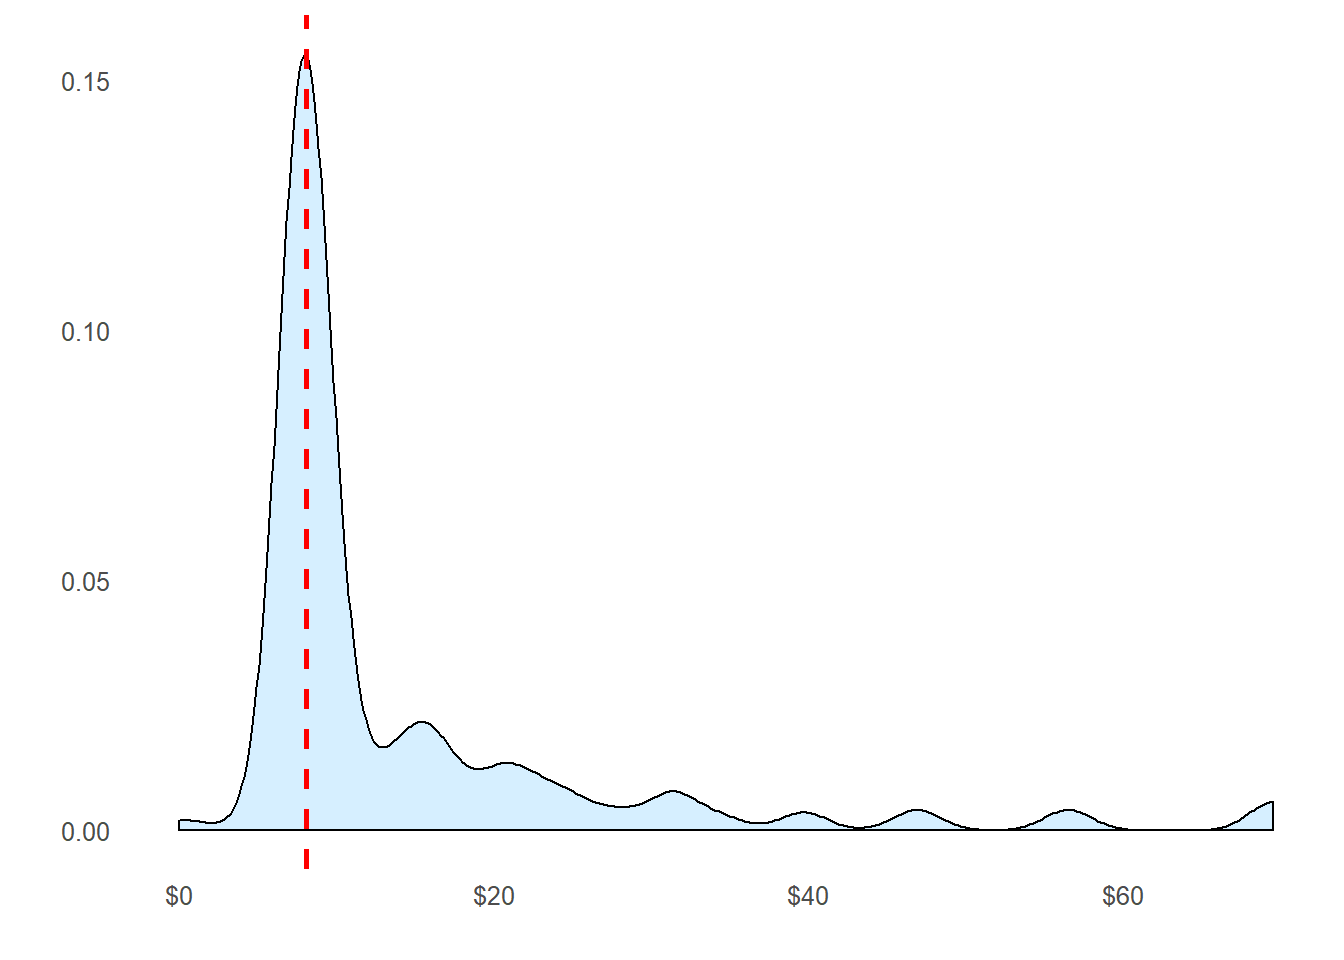
\includegraphics{15-Feature_files/figure-latex/unnamed-chunk-6-1.pdf}

Ah hah. We can see that there's a survival penalty to singletons and
those with family sizes above 4. We can collapse this variable into
three levels which will be helpful since there are comparatively fewer
large families. Let's create a discretized family size variable.

\begin{Shaded}
\begin{Highlighting}[]
\CommentTok{# Discretize family size}
\NormalTok{full}\OperatorTok{$}\NormalTok{FsizeD[full}\OperatorTok{$}\NormalTok{Fsize }\OperatorTok{==}\StringTok{ }\DecValTok{1}\NormalTok{] <-}\StringTok{ 'singleton'}
\NormalTok{full}\OperatorTok{$}\NormalTok{FsizeD[full}\OperatorTok{$}\NormalTok{Fsize }\OperatorTok{<}\StringTok{ }\DecValTok{5} \OperatorTok{&}\StringTok{ }\NormalTok{full}\OperatorTok{$}\NormalTok{Fsize }\OperatorTok{>}\StringTok{ }\DecValTok{1}\NormalTok{] <-}\StringTok{ 'small'}
\NormalTok{full}\OperatorTok{$}\NormalTok{FsizeD[full}\OperatorTok{$}\NormalTok{Fsize }\OperatorTok{>}\StringTok{ }\DecValTok{4}\NormalTok{] <-}\StringTok{ 'large'}

\CommentTok{# Show family size by survival using a mosaic plot}
\KeywordTok{mosaicplot}\NormalTok{(}\KeywordTok{table}\NormalTok{(full}\OperatorTok{$}\NormalTok{FsizeD, full}\OperatorTok{$}\NormalTok{Survived), }\DataTypeTok{main=}\StringTok{'Family Size by Survival'}\NormalTok{, }\DataTypeTok{shade=}\OtherTok{TRUE}\NormalTok{)}
\end{Highlighting}
\end{Shaded}

\includegraphics{15-Feature_files/figure-latex/unnamed-chunk-7-1.pdf}
The mosaic plot shows that we preserve our rule that there's a survival
penalty among singletons and large families, but a benefit for
passengers in small families. I want to do something further with our
age variable, but 263 rows have missing age values, so we will have to
wait until after we address missingness.

\subsection{Treat a few more variables
\ldots{}}\label{treat-a-few-more-variables}

What's left? There's probably some potentially useful information in the
passenger cabin variable including about their deck. Let's take a look.

\begin{Shaded}
\begin{Highlighting}[]
\CommentTok{# This variable appears to have a lot of missing values}
\NormalTok{full}\OperatorTok{$}\NormalTok{Cabin[}\DecValTok{1}\OperatorTok{:}\DecValTok{28}\NormalTok{]}
\end{Highlighting}
\end{Shaded}

\begin{verbatim}
##  [1] ""            "C85"         ""            "C123"        ""           
##  [6] ""            "E46"         ""            ""            ""           
## [11] "G6"          "C103"        ""            ""            ""           
## [16] ""            ""            ""            ""            ""           
## [21] ""            "D56"         ""            "A6"          ""           
## [26] ""            ""            "C23 C25 C27"
\end{verbatim}

\begin{Shaded}
\begin{Highlighting}[]
\CommentTok{# The first character is the deck. For example:}
\KeywordTok{strsplit}\NormalTok{(full}\OperatorTok{$}\NormalTok{Cabin[}\DecValTok{2}\NormalTok{], }\OtherTok{NULL}\NormalTok{)[[}\DecValTok{1}\NormalTok{]]}
\end{Highlighting}
\end{Shaded}

\begin{verbatim}
## [1] "C" "8" "5"
\end{verbatim}

\begin{Shaded}
\begin{Highlighting}[]
\CommentTok{# Create a Deck variable. Get passenger deck A - F:}
\NormalTok{full}\OperatorTok{$}\NormalTok{Deck<-}\KeywordTok{factor}\NormalTok{(}\KeywordTok{sapply}\NormalTok{(full}\OperatorTok{$}\NormalTok{Cabin, }\ControlFlowTok{function}\NormalTok{(x) }\KeywordTok{strsplit}\NormalTok{(x, }\OtherTok{NULL}\NormalTok{)[[}\DecValTok{1}\NormalTok{]][}\DecValTok{1}\NormalTok{]))}
\end{Highlighting}
\end{Shaded}

There's more that likely could be done here including looking into
cabins with multiple rooms listed (e.g., row 28: ``C23 C25 C27''), but
given the sparseness of the column we'll stop here.

\section{Missingness}\label{missingness}

Now we're ready to start exploring missing data and rectifying it
through imputation. There are a number of different ways we could go
about doing this. Given the small size of the dataset, we probably
should not opt for deleting either entire observations (rows) or
variables (columns) containing missing values. We're left with the
option of either replacing missing values with a sensible values given
the distribution of the data, e.g., the mean, median or mode. Finally,
we could go with prediction. We'll use both of the two latter methods
and I'll rely on some data visualization to guide our decisions.

\subsection{Sensible value imputation}\label{sensible-value-imputation}

\begin{Shaded}
\begin{Highlighting}[]
\CommentTok{# Passengers 62 and 830 are missing Embarkment}
\NormalTok{full[}\KeywordTok{c}\NormalTok{(}\DecValTok{62}\NormalTok{, }\DecValTok{830}\NormalTok{), }\StringTok{'Embarked'}\NormalTok{]}
\end{Highlighting}
\end{Shaded}

\begin{verbatim}
## [1] "" ""
\end{verbatim}

\begin{verbatim}
## We will infer their values for **embarkment** based on present data that we can imagine may be relevant: **passenger class** and **fare**. We see that they paid<b> $ 80 </b>and<b> $ NA </b>respectively and their classes are<b> 1 </b>and<b> NA </b>. So from where did they embark?
\end{verbatim}

\begin{Shaded}
\begin{Highlighting}[]
\CommentTok{# Get rid of our missing passenger IDs}
\NormalTok{embark_fare <-}\StringTok{ }\NormalTok{full }\OperatorTok
\StringTok{  }\KeywordTok{filter}\NormalTok{(PassengerId }\OperatorTok{!=}\StringTok{ }\DecValTok{62} \OperatorTok{&}\StringTok{ }\NormalTok{PassengerId }\OperatorTok{!=}\StringTok{ }\DecValTok{830}\NormalTok{)}

\CommentTok{# Use ggplot2 to visualize embarkment, passenger class, & median fare}
\KeywordTok{ggplot}\NormalTok{(embark_fare, }\KeywordTok{aes}\NormalTok{(}\DataTypeTok{x =}\NormalTok{ Embarked, }\DataTypeTok{y =}\NormalTok{ Fare, }\DataTypeTok{fill =} \KeywordTok{factor}\NormalTok{(Pclass))) }\OperatorTok{+}
\StringTok{  }\KeywordTok{geom_boxplot}\NormalTok{() }\OperatorTok{+}
\StringTok{  }\KeywordTok{geom_hline}\NormalTok{(}\KeywordTok{aes}\NormalTok{(}\DataTypeTok{yintercept=}\DecValTok{80}\NormalTok{), }
    \DataTypeTok{colour=}\StringTok{'red'}\NormalTok{, }\DataTypeTok{linetype=}\StringTok{'dashed'}\NormalTok{, }\DataTypeTok{lwd=}\DecValTok{2}\NormalTok{) }\OperatorTok{+}
\StringTok{  }\KeywordTok{scale_y_continuous}\NormalTok{(}\DataTypeTok{labels=}\KeywordTok{dollar_format}\NormalTok{()) }\OperatorTok{+}
\StringTok{  }\KeywordTok{theme_few}\NormalTok{()}
\end{Highlighting}
\end{Shaded}

\includegraphics{16-Missingness_files/figure-latex/unnamed-chunk-4-1.pdf}
Voilà! The median fare for a first class passenger departing from
Charbourg (`C') coincides nicely with the \$80 paid by our
embarkment-deficient passengers. I think we can safely replace the NA
values with `C'.

\begin{Shaded}
\begin{Highlighting}[]
\CommentTok{# Since their fare was $80 for 1st class, they most likely embarked from 'C'}
\NormalTok{full}\OperatorTok{$}\NormalTok{Embarked[}\KeywordTok{c}\NormalTok{(}\DecValTok{62}\NormalTok{, }\DecValTok{830}\NormalTok{)] <-}\StringTok{ 'C'}
\end{Highlighting}
\end{Shaded}

We're close to fixing the handful of NA values here and there. Passenger
on row 1044 has an NA Fare value.

\begin{Shaded}
\begin{Highlighting}[]
\CommentTok{# Show row 1044}
\NormalTok{full[}\DecValTok{1044}\NormalTok{, ]}
\end{Highlighting}
\end{Shaded}

\begin{verbatim}
##      PassengerId Survived Pclass               Name  Sex  Age SibSp Parch
## 1044        1044       NA      3 Storey, Mr. Thomas male 60.5     0     0
##      Ticket Fare Cabin Embarked Title Surname Fsize   Family    FsizeD
## 1044   3701   NA              S    Mr  Storey     1 Storey_1 singleton
##      Deck
## 1044 <NA>
\end{verbatim}

This is a third class passenger who departed from Southampton (`S').
Let's visualize Fares among all others sharing their class and
embarkment (n = 494).

\begin{Shaded}
\begin{Highlighting}[]
\KeywordTok{ggplot}\NormalTok{(full[full}\OperatorTok{$}\NormalTok{Pclass }\OperatorTok{==}\StringTok{ '3'} \OperatorTok{&}\StringTok{ }\NormalTok{full}\OperatorTok{$}\NormalTok{Embarked }\OperatorTok{==}\StringTok{ 'S'}\NormalTok{, ], }
  \KeywordTok{aes}\NormalTok{(}\DataTypeTok{x =}\NormalTok{ Fare)) }\OperatorTok{+}
\StringTok{  }\KeywordTok{geom_density}\NormalTok{(}\DataTypeTok{fill =} \StringTok{'#99d6ff'}\NormalTok{, }\DataTypeTok{alpha=}\FloatTok{0.4}\NormalTok{) }\OperatorTok{+}\StringTok{ }
\StringTok{  }\KeywordTok{geom_vline}\NormalTok{(}\KeywordTok{aes}\NormalTok{(}\DataTypeTok{xintercept=}\KeywordTok{median}\NormalTok{(Fare, }\DataTypeTok{na.rm=}\NormalTok{T)),}
    \DataTypeTok{colour=}\StringTok{'red'}\NormalTok{, }\DataTypeTok{linetype=}\StringTok{'dashed'}\NormalTok{, }\DataTypeTok{lwd=}\DecValTok{1}\NormalTok{) }\OperatorTok{+}
\StringTok{  }\KeywordTok{scale_x_continuous}\NormalTok{(}\DataTypeTok{labels=}\KeywordTok{dollar_format}\NormalTok{()) }\OperatorTok{+}
\StringTok{  }\KeywordTok{theme_few}\NormalTok{()}
\end{Highlighting}
\end{Shaded}

\includegraphics{16-Missingness_files/figure-latex/unnamed-chunk-7-1.pdf}

From this visualization, it seems quite reasonable to replace the NA
Fare value with median for their class and embarkment which is \$8.05.

\begin{Shaded}
\begin{Highlighting}[]
\CommentTok{# Replace missing fare value with median fare for class/embarkment}
\NormalTok{full}\OperatorTok{$}\NormalTok{Fare[}\DecValTok{1044}\NormalTok{] <-}\StringTok{ }\KeywordTok{median}\NormalTok{(full[full}\OperatorTok{$}\NormalTok{Pclass }\OperatorTok{==}\StringTok{ '3'} \OperatorTok{&}\StringTok{ }\NormalTok{full}\OperatorTok{$}\NormalTok{Embarked }\OperatorTok{==}\StringTok{ 'S'}\NormalTok{, ]}\OperatorTok{$}\NormalTok{Fare, }\DataTypeTok{na.rm =} \OtherTok{TRUE}\NormalTok{)}
\end{Highlighting}
\end{Shaded}

\subsection{Predictive imputation}\label{predictive-imputation}

Finally, as we noted earlier, there are quite a few missing Age values
in our data. We are going to get a bit more fancy in imputing missing
age values. Why? Because we can. We will create a model predicting ages
based on other variables.

\begin{Shaded}
\begin{Highlighting}[]
\CommentTok{# Show number of missing Age values}
\KeywordTok{sum}\NormalTok{(}\KeywordTok{is.na}\NormalTok{(full}\OperatorTok{$}\NormalTok{Age))}
\end{Highlighting}
\end{Shaded}

\begin{verbatim}
## [1] 263
\end{verbatim}

We could definitely use rpart (recursive partitioning for regression) to
predict missing ages, but I'm going to use the mice package for this
task just for something different. You can read more about multiple
imputation using chained equations in r here (PDF). Since we haven't
done it yet, I'll first factorize the factor variables and then perform
mice imputation.

\begin{Shaded}
\begin{Highlighting}[]
\CommentTok{# Make variables factors into factors}
\NormalTok{factor_vars <-}\StringTok{ }\KeywordTok{c}\NormalTok{(}\StringTok{'PassengerId'}\NormalTok{,}\StringTok{'Pclass'}\NormalTok{,}\StringTok{'Sex'}\NormalTok{,}\StringTok{'Embarked'}\NormalTok{,}
                 \StringTok{'Title'}\NormalTok{,}\StringTok{'Surname'}\NormalTok{,}\StringTok{'Family'}\NormalTok{,}\StringTok{'FsizeD'}\NormalTok{)}

\NormalTok{full[factor_vars] <-}\StringTok{ }\KeywordTok{lapply}\NormalTok{(full[factor_vars], }\ControlFlowTok{function}\NormalTok{(x) }\KeywordTok{as.factor}\NormalTok{(x))}

\CommentTok{# Set a random seed}
\KeywordTok{set.seed}\NormalTok{(}\DecValTok{129}\NormalTok{)}

\CommentTok{# Perform mice imputation, excluding certain less-than-useful variables:}
\NormalTok{mice_mod <-}\StringTok{ }\KeywordTok{mice}\NormalTok{(full[, }\OperatorTok{!}\KeywordTok{names}\NormalTok{(full) }\OperatorTok\StringTok{ }\KeywordTok{c}\NormalTok{(}\StringTok{'PassengerId'}\NormalTok{,}\StringTok{'Name'}\NormalTok{,}\StringTok{'Ticket'}\NormalTok{,}\StringTok{'Cabin'}\NormalTok{,}\StringTok{'Family'}\NormalTok{,}\StringTok{'Surname'}\NormalTok{,}\StringTok{'Survived'}\NormalTok{)], }\DataTypeTok{method=}\StringTok{'rf'}\NormalTok{) }
\end{Highlighting}
\end{Shaded}

\begin{verbatim}
## 
##  iter imp variable
##   1   1  Age  Deck
##   1   2  Age  Deck
##   1   3  Age  Deck
##   1   4  Age  Deck
##   1   5  Age  Deck
##   2   1  Age  Deck
##   2   2  Age  Deck
##   2   3  Age  Deck
##   2   4  Age  Deck
##   2   5  Age  Deck
##   3   1  Age  Deck
##   3   2  Age  Deck
##   3   3  Age  Deck
##   3   4  Age  Deck
##   3   5  Age  Deck
##   4   1  Age  Deck
##   4   2  Age  Deck
##   4   3  Age  Deck
##   4   4  Age  Deck
##   4   5  Age  Deck
##   5   1  Age  Deck
##   5   2  Age  Deck
##   5   3  Age  Deck
##   5   4  Age  Deck
##   5   5  Age  Deck
\end{verbatim}

\begin{Shaded}
\begin{Highlighting}[]
\CommentTok{# Save the complete output }
\NormalTok{mice_output <-}\StringTok{ }\KeywordTok{complete}\NormalTok{(mice_mod)}
\end{Highlighting}
\end{Shaded}

Let's compare the results we get with the original distribution of
passenger ages to ensure that nothing has gone completely awry.

\begin{Shaded}
\begin{Highlighting}[]
\CommentTok{# Plot age distributions}
\KeywordTok{par}\NormalTok{(}\DataTypeTok{mfrow=}\KeywordTok{c}\NormalTok{(}\DecValTok{1}\NormalTok{,}\DecValTok{2}\NormalTok{))}
\KeywordTok{hist}\NormalTok{(full}\OperatorTok{$}\NormalTok{Age, }\DataTypeTok{freq=}\NormalTok{F, }\DataTypeTok{main=}\StringTok{'Age: Original Data'}\NormalTok{, }
  \DataTypeTok{col=}\StringTok{'darkgreen'}\NormalTok{, }\DataTypeTok{ylim=}\KeywordTok{c}\NormalTok{(}\DecValTok{0}\NormalTok{,}\FloatTok{0.04}\NormalTok{))}
\KeywordTok{hist}\NormalTok{(mice_output}\OperatorTok{$}\NormalTok{Age, }\DataTypeTok{freq=}\NormalTok{F, }\DataTypeTok{main=}\StringTok{'Age: MICE Output'}\NormalTok{, }
  \DataTypeTok{col=}\StringTok{'lightgreen'}\NormalTok{, }\DataTypeTok{ylim=}\KeywordTok{c}\NormalTok{(}\DecValTok{0}\NormalTok{,}\FloatTok{0.04}\NormalTok{))}
\end{Highlighting}
\end{Shaded}

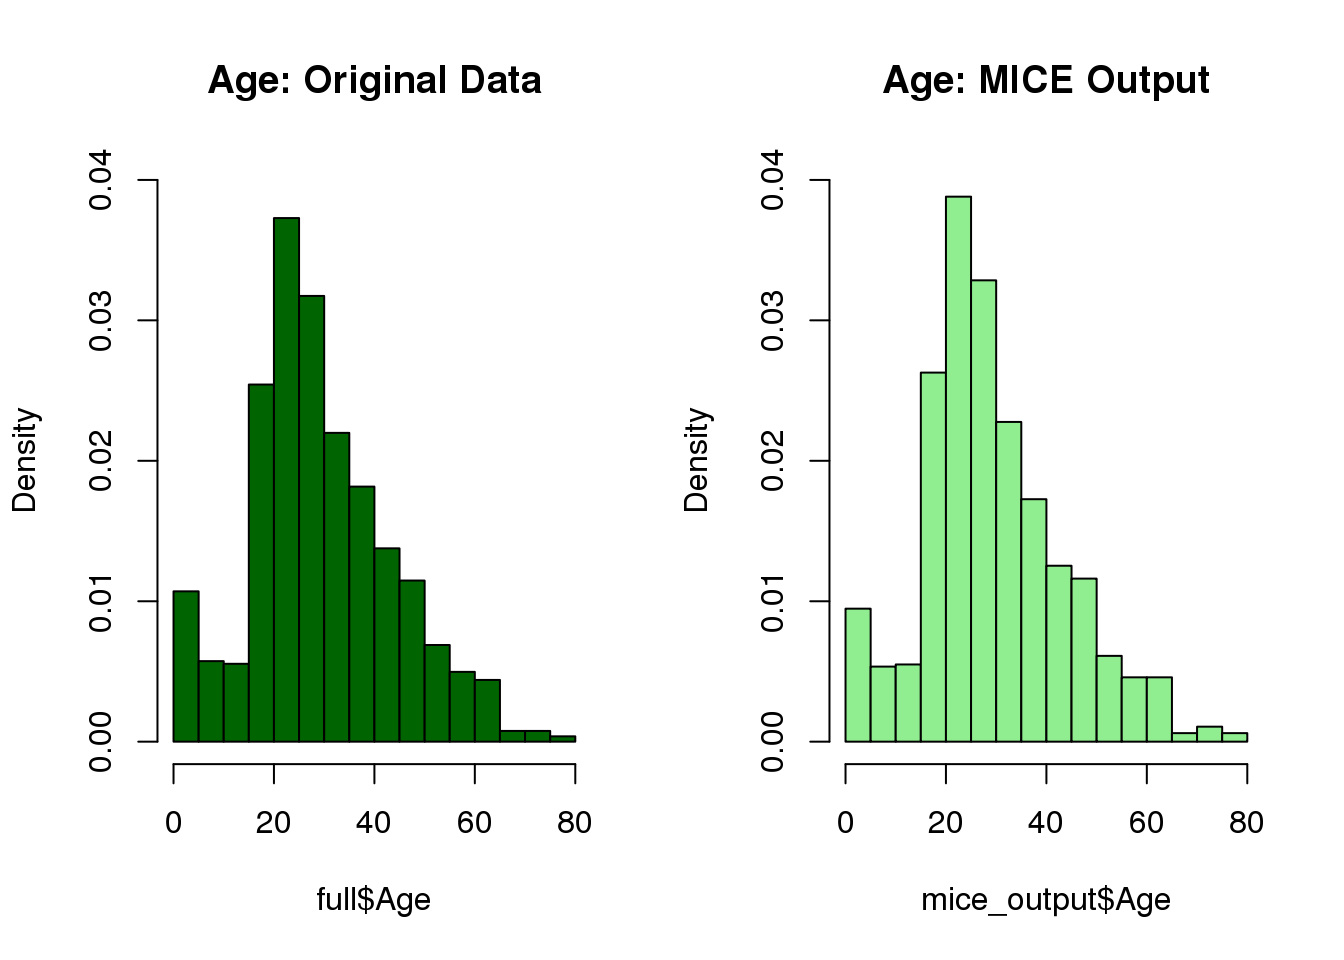
\includegraphics{16-Missingness_files/figure-latex/unnamed-chunk-12-1.pdf}

Things look good, so let's replace our age vector in the original data
with the output from the mice model.

\begin{Shaded}
\begin{Highlighting}[]
\CommentTok{# Replace Age variable from the mice model.}
\NormalTok{full}\OperatorTok{$}\NormalTok{Age <-}\StringTok{ }\NormalTok{mice_output}\OperatorTok{$}\NormalTok{Age}

\CommentTok{# Show new number of missing Age values}
\KeywordTok{sum}\NormalTok{(}\KeywordTok{is.na}\NormalTok{(full}\OperatorTok{$}\NormalTok{Age))}
\end{Highlighting}
\end{Shaded}

\begin{verbatim}
## [1] 0
\end{verbatim}

We've finished imputing values for all variables that we care about for
now! Now that we have a complete Age variable, there are just a few
finishing touches I'd like to make. We can use Age to do just a bit more
feature engineering \ldots{}

\subsection{Feature Engineering: Round
2}\label{feature-engineering-round-2}

Now that we know everyone's age, we can create a couple of new
age-dependent variables: Child and Mother. A child will simply be
someone under 18 years of age and a mother is a passenger who is 1)
female, 2) is over 18, 3) has more than 0 children (no kidding!), and 4)
does not have the title `Miss'.

\begin{Shaded}
\begin{Highlighting}[]
\CommentTok{# First we'll look at the relationship between age & survival}
\KeywordTok{ggplot}\NormalTok{(full[}\DecValTok{1}\OperatorTok{:}\DecValTok{891}\NormalTok{,], }\KeywordTok{aes}\NormalTok{(Age, }\DataTypeTok{fill =} \KeywordTok{factor}\NormalTok{(Survived))) }\OperatorTok{+}\StringTok{ }
\StringTok{  }\KeywordTok{geom_histogram}\NormalTok{() }\OperatorTok{+}\StringTok{ }
\StringTok{  }\CommentTok{# I include Sex since we know (a priori) it's a significant predictor}
\StringTok{  }\KeywordTok{facet_grid}\NormalTok{(.}\OperatorTok{~}\NormalTok{Sex) }\OperatorTok{+}\StringTok{ }
\StringTok{  }\KeywordTok{theme_few}\NormalTok{()}
\end{Highlighting}
\end{Shaded}

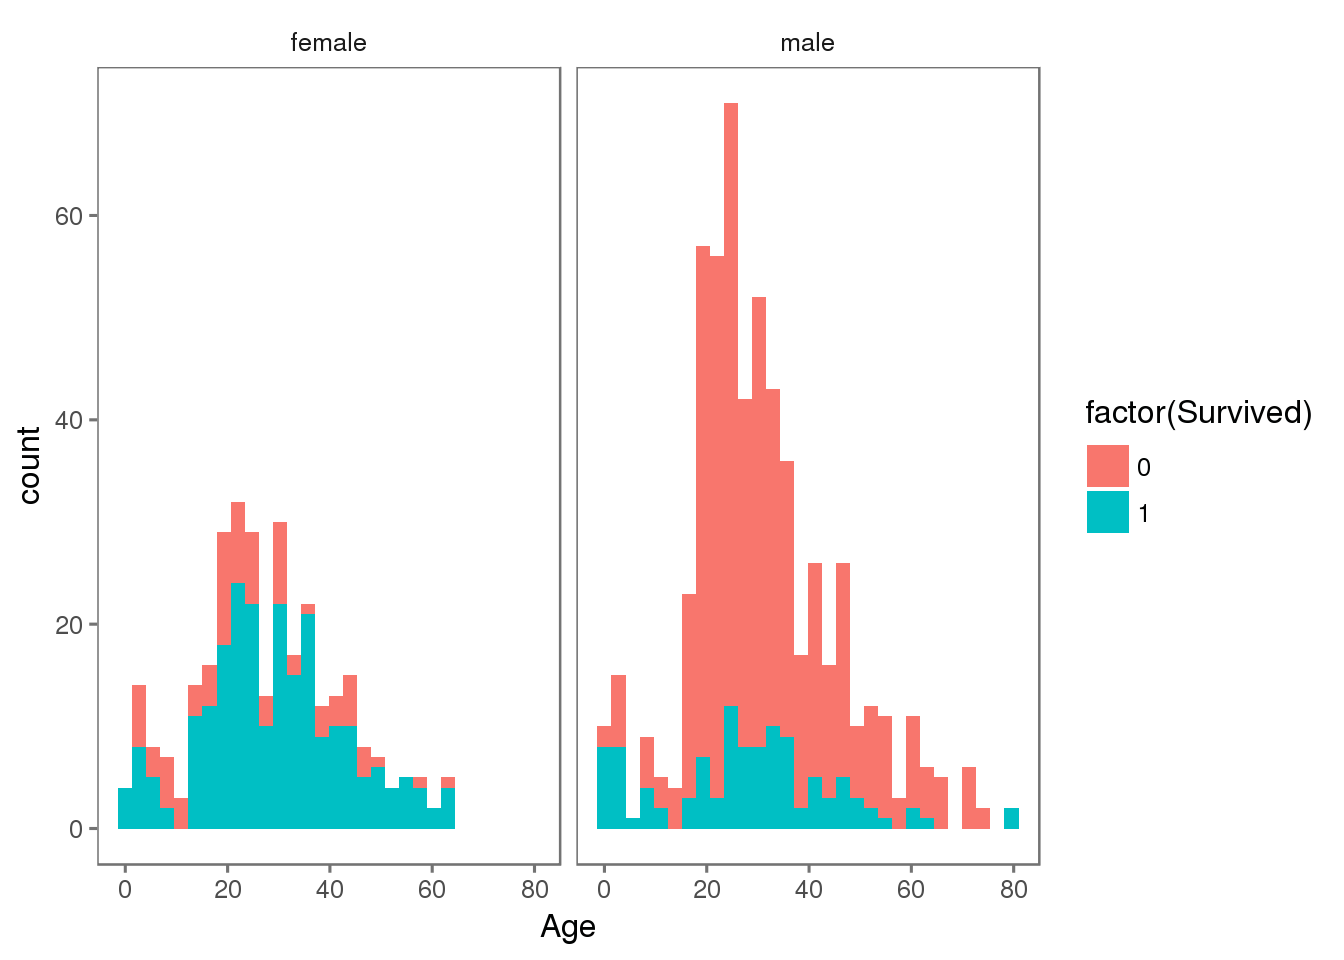
\includegraphics{16-Missingness_files/figure-latex/unnamed-chunk-14-1.pdf}

\begin{Shaded}
\begin{Highlighting}[]
\CommentTok{# Create the column child, and indicate whether child or adult}
\NormalTok{full}\OperatorTok{$}\NormalTok{Child[full}\OperatorTok{$}\NormalTok{Age }\OperatorTok{<}\StringTok{ }\DecValTok{18}\NormalTok{] <-}\StringTok{ 'Child'}
\NormalTok{full}\OperatorTok{$}\NormalTok{Child[full}\OperatorTok{$}\NormalTok{Age }\OperatorTok{>=}\StringTok{ }\DecValTok{18}\NormalTok{] <-}\StringTok{ 'Adult'}

\CommentTok{# Show counts}
\KeywordTok{table}\NormalTok{(full}\OperatorTok{$}\NormalTok{Child, full}\OperatorTok{$}\NormalTok{Survived)}
\end{Highlighting}
\end{Shaded}

\begin{verbatim}
##        
##           0   1
##   Adult 484 274
##   Child  65  68
\end{verbatim}

Looks like being a child doesn't hurt, but it's not going to necessarily
save you either! We will finish off our feature engineering by creating
the Mother variable. Maybe we can hope that mothers are more likely to
have survived on the Titanic.

\begin{Shaded}
\begin{Highlighting}[]
\CommentTok{# Adding Mother variable}
\NormalTok{full}\OperatorTok{$}\NormalTok{Mother <-}\StringTok{ 'Not Mother'}
\NormalTok{full}\OperatorTok{$}\NormalTok{Mother[full}\OperatorTok{$}\NormalTok{Sex }\OperatorTok{==}\StringTok{ 'female'} \OperatorTok{&}\StringTok{ }\NormalTok{full}\OperatorTok{$}\NormalTok{Parch }\OperatorTok{>}\StringTok{ }\DecValTok{0} \OperatorTok{&}\StringTok{ }\NormalTok{full}\OperatorTok{$}\NormalTok{Age }\OperatorTok{>}\StringTok{ }\DecValTok{18} \OperatorTok{&}\StringTok{ }\NormalTok{full}\OperatorTok{$}\NormalTok{Title }\OperatorTok{!=}\StringTok{ 'Miss'}\NormalTok{] <-}\StringTok{ 'Mother'}

\CommentTok{# Show counts}
\KeywordTok{table}\NormalTok{(full}\OperatorTok{$}\NormalTok{Mother, full}\OperatorTok{$}\NormalTok{Survived)}
\end{Highlighting}
\end{Shaded}

\begin{verbatim}
##             
##                0   1
##   Mother      16  39
##   Not Mother 533 303
\end{verbatim}

\begin{Shaded}
\begin{Highlighting}[]
\CommentTok{# Finish by factorizing our two new factor variables}
\NormalTok{full}\OperatorTok{$}\NormalTok{Child  <-}\StringTok{ }\KeywordTok{factor}\NormalTok{(full}\OperatorTok{$}\NormalTok{Child)}
\NormalTok{full}\OperatorTok{$}\NormalTok{Mother <-}\StringTok{ }\KeywordTok{factor}\NormalTok{(full}\OperatorTok{$}\NormalTok{Mother)}
\end{Highlighting}
\end{Shaded}

All of the variables we care about should be taken care of and there
should be no missing data. I'm going to double check just to be sure:

\begin{Shaded}
\begin{Highlighting}[]
\KeywordTok{md.pattern}\NormalTok{(full)}
\end{Highlighting}
\end{Shaded}

\begin{verbatim}
## Warning in data.matrix(x): NAs introduced by coercion

## Warning in data.matrix(x): NAs introduced by coercion

## Warning in data.matrix(x): NAs introduced by coercion
\end{verbatim}

\begin{verbatim}
##     PassengerId Pclass Sex Age SibSp Parch Fare Embarked Title Surname
## 150           1      1   1   1     1     1    1        1     1       1
##  61           1      1   1   1     1     1    1        1     1       1
##  54           1      1   1   1     1     1    1        1     1       1
## 511           1      1   1   1     1     1    1        1     1       1
##  30           1      1   1   1     1     1    1        1     1       1
## 235           1      1   1   1     1     1    1        1     1       1
## 176           1      1   1   1     1     1    1        1     1       1
##  92           1      1   1   1     1     1    1        1     1       1
##               0      0   0   0     0     0    0        0     0       0
##     Fsize Family FsizeD Child Mother Ticket Survived Deck Name Cabin     
## 150     1      1      1     1      1      1        1    1    0     0    2
##  61     1      1      1     1      1      1        0    1    0     0    3
##  54     1      1      1     1      1      0        1    1    0     0    3
## 511     1      1      1     1      1      1        1    0    0     0    3
##  30     1      1      1     1      1      0        0    1    0     0    4
## 235     1      1      1     1      1      1        0    0    0     0    4
## 176     1      1      1     1      1      0        1    0    0     0    4
##  92     1      1      1     1      1      0        0    0    0     0    5
##         0      0      0     0      0    352      418 1014 1309  1309 4402
\end{verbatim}

Wow! We have finally finished treating all of the relevant missing
values in the Titanic dataset which has included some fancy imputation
with mice. We have also successfully created several new variables which
we hope will help us build a model which reliably predicts survival.

\section{Prediction}\label{prediction}

At last we're ready to predict who survives among passengers of the
Titanic based on variables that we carefully curated and treated for
missing values. For this, we will rely on the randomForest
classification algorithm; we spent all that time on imputation, after
all.

\subsection{Split into training \& test
sets}\label{split-into-training-test-sets}

Our first step is to split the data back into the original test and
training sets.

\begin{Shaded}
\begin{Highlighting}[]
\CommentTok{# Split the data back into a train set and a test set}
\NormalTok{train <-}\StringTok{ }\NormalTok{full[}\DecValTok{1}\OperatorTok{:}\DecValTok{891}\NormalTok{,]}
\NormalTok{test <-}\StringTok{ }\NormalTok{full[}\DecValTok{892}\OperatorTok{:}\DecValTok{1309}\NormalTok{,]}
\end{Highlighting}
\end{Shaded}

\subsection{Building the model}\label{building-the-model}

We then build our model using randomForest on the training set.

\begin{Shaded}
\begin{Highlighting}[]
\CommentTok{# Set a random seed}
\KeywordTok{set.seed}\NormalTok{(}\DecValTok{754}\NormalTok{)}

\CommentTok{# Build the model (note: not all possible variables are used)}
\NormalTok{rf_model <-}\StringTok{ }\KeywordTok{randomForest}\NormalTok{(}\KeywordTok{factor}\NormalTok{(Survived) }\OperatorTok{~}\StringTok{ }\NormalTok{Pclass }\OperatorTok{+}\StringTok{ }\NormalTok{Sex }\OperatorTok{+}\StringTok{ }\NormalTok{Age }\OperatorTok{+}\StringTok{ }\NormalTok{SibSp }\OperatorTok{+}\StringTok{ }\NormalTok{Parch }\OperatorTok{+}\StringTok{ }
\StringTok{                                            }\NormalTok{Fare }\OperatorTok{+}\StringTok{ }\NormalTok{Embarked }\OperatorTok{+}\StringTok{ }\NormalTok{Title }\OperatorTok{+}\StringTok{ }
\StringTok{                                            }\NormalTok{FsizeD }\OperatorTok{+}\StringTok{ }\NormalTok{Child }\OperatorTok{+}\StringTok{ }\NormalTok{Mother,}
                                            \DataTypeTok{data =}\NormalTok{ train)}

\CommentTok{# Show model error}
\KeywordTok{plot}\NormalTok{(rf_model, }\DataTypeTok{ylim=}\KeywordTok{c}\NormalTok{(}\DecValTok{0}\NormalTok{,}\FloatTok{0.36}\NormalTok{))}
\KeywordTok{legend}\NormalTok{(}\StringTok{'topright'}\NormalTok{, }\KeywordTok{colnames}\NormalTok{(rf_model}\OperatorTok{$}\NormalTok{err.rate), }\DataTypeTok{col=}\DecValTok{1}\OperatorTok{:}\DecValTok{3}\NormalTok{, }\DataTypeTok{fill=}\DecValTok{1}\OperatorTok{:}\DecValTok{3}\NormalTok{)}
\end{Highlighting}
\end{Shaded}

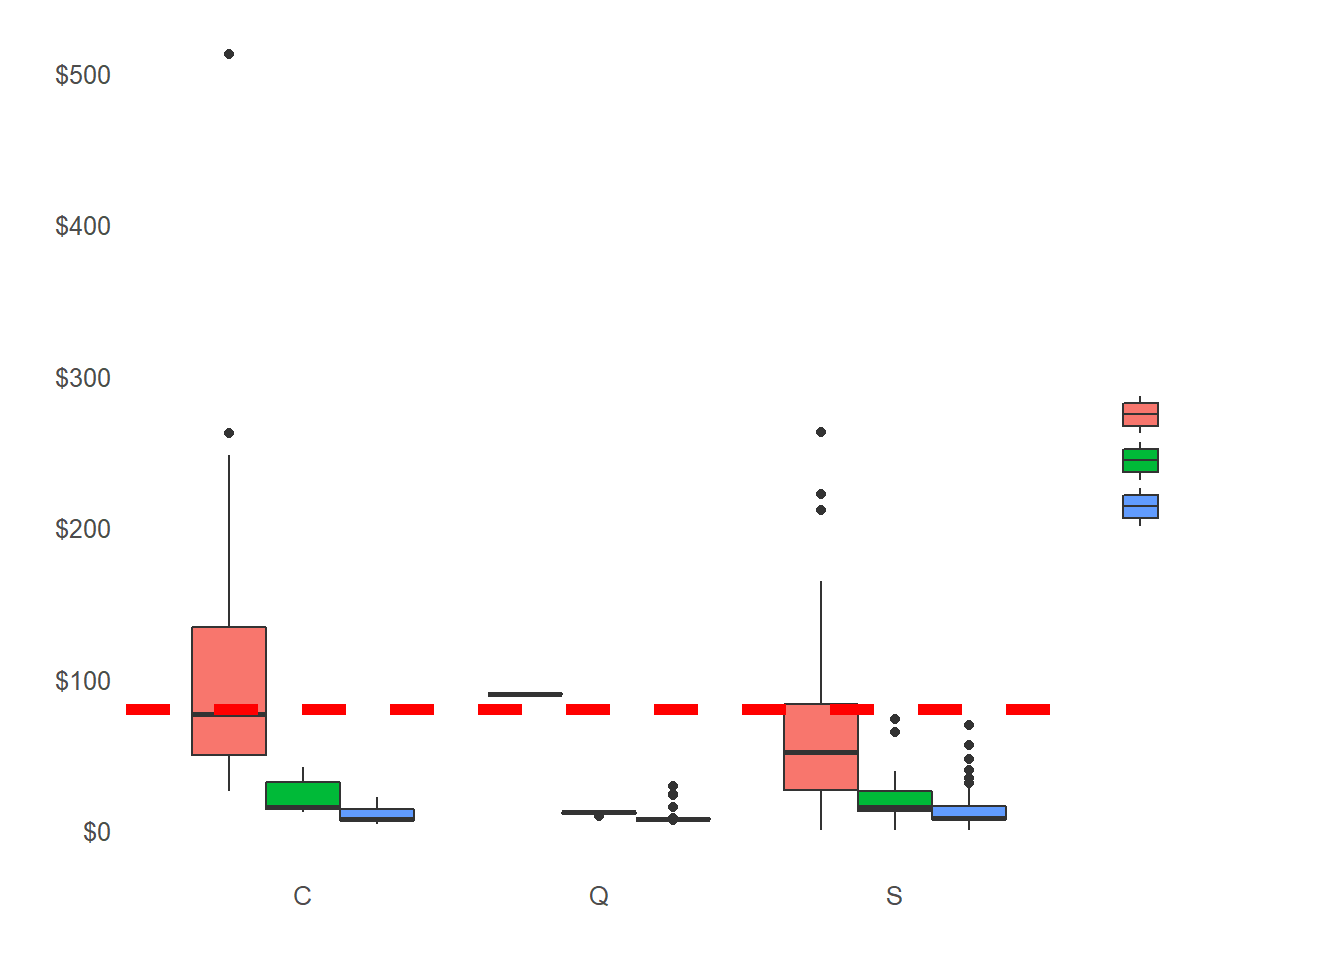
\includegraphics{17-Prediction_files/figure-latex/unnamed-chunk-3-1.pdf}

The black line shows the overall error rate which falls below 20\%. The
red and green lines show the error rate for `died' and `survived'
respectively. We can see that right now we're much more successful
predicting death than we are survival. What does that say about me, I
wonder?

\subsection{Variable importance}\label{variable-importance}

Let's look at relative variable importance by plotting the mean decrease
in Gini calculated across all trees.

\begin{Shaded}
\begin{Highlighting}[]
\CommentTok{# Get importance}
\NormalTok{importance    <-}\StringTok{ }\KeywordTok{importance}\NormalTok{(rf_model)}
\NormalTok{varImportance <-}\StringTok{ }\KeywordTok{data.frame}\NormalTok{(}\DataTypeTok{Variables =} \KeywordTok{row.names}\NormalTok{(importance), }
                            \DataTypeTok{Importance =} \KeywordTok{round}\NormalTok{(importance[ ,}\StringTok{'MeanDecreaseGini'}\NormalTok{],}\DecValTok{2}\NormalTok{))}

\CommentTok{# Create a rank variable based on importance}
\NormalTok{rankImportance <-}\StringTok{ }\NormalTok{varImportance }\OperatorTok
\StringTok{  }\KeywordTok{mutate}\NormalTok{(}\DataTypeTok{Rank =} \KeywordTok{paste0}\NormalTok{(}\StringTok{'#'}\NormalTok{,}\KeywordTok{dense_rank}\NormalTok{(}\KeywordTok{desc}\NormalTok{(Importance))))}

\CommentTok{# Use ggplot2 to visualize the relative importance of variables}
\KeywordTok{ggplot}\NormalTok{(rankImportance, }\KeywordTok{aes}\NormalTok{(}\DataTypeTok{x =} \KeywordTok{reorder}\NormalTok{(Variables, Importance), }
    \DataTypeTok{y =}\NormalTok{ Importance, }\DataTypeTok{fill =}\NormalTok{ Importance)) }\OperatorTok{+}
\StringTok{  }\KeywordTok{geom_bar}\NormalTok{(}\DataTypeTok{stat=}\StringTok{'identity'}\NormalTok{) }\OperatorTok{+}\StringTok{ }
\StringTok{  }\KeywordTok{geom_text}\NormalTok{(}\KeywordTok{aes}\NormalTok{(}\DataTypeTok{x =}\NormalTok{ Variables, }\DataTypeTok{y =} \FloatTok{0.5}\NormalTok{, }\DataTypeTok{label =}\NormalTok{ Rank),}
    \DataTypeTok{hjust=}\DecValTok{0}\NormalTok{, }\DataTypeTok{vjust=}\FloatTok{0.55}\NormalTok{, }\DataTypeTok{size =} \DecValTok{4}\NormalTok{, }\DataTypeTok{colour =} \StringTok{'red'}\NormalTok{) }\OperatorTok{+}
\StringTok{  }\KeywordTok{labs}\NormalTok{(}\DataTypeTok{x =} \StringTok{'Variables'}\NormalTok{) }\OperatorTok{+}
\StringTok{  }\KeywordTok{coord_flip}\NormalTok{() }\OperatorTok{+}\StringTok{ }
\StringTok{  }\KeywordTok{theme_few}\NormalTok{()}
\end{Highlighting}
\end{Shaded}

\includegraphics{17-Prediction_files/figure-latex/unnamed-chunk-4-1.pdf}

Whoa, glad we made our title variable! It has the highest relative
importance out of all of our predictor variables. I think I'm most
surprised to see that passenger class fell to \#5, but maybe that's just
bias coming from watching the movie Titanic too many times as a kid.

\subsection{Prediction!}\label{prediction-1}

We're ready for the final step --- making our prediction! When we finish
here, we could iterate through the preceding steps making tweaks as we
go or fit the data using different models or use different combinations
of variables to achieve better predictions. But this is a good starting
(and stopping) point for me now.

\begin{Shaded}
\begin{Highlighting}[]
\CommentTok{# Predict using the test set}
\NormalTok{prediction <-}\StringTok{ }\KeywordTok{predict}\NormalTok{(rf_model, test)}

\CommentTok{# Save the solution to a dataframe with two columns: PassengerId and Survived (prediction)}
\NormalTok{solution <-}\StringTok{ }\KeywordTok{data.frame}\NormalTok{(}\DataTypeTok{PassengerID =}\NormalTok{ test}\OperatorTok{$}\NormalTok{PassengerId, }\DataTypeTok{Survived =}\NormalTok{ prediction)}

\CommentTok{# Write the solution to file}
\KeywordTok{write.csv}\NormalTok{(solution, }\DataTypeTok{file =} \StringTok{'rf_mod_Solution.csv'}\NormalTok{, }\DataTypeTok{row.names =}\NormalTok{ F)}
\end{Highlighting}
\end{Shaded}

\bibliography{book.bib}


\end{document}
